\documentclass[14,fleqn]{article}
\usepackage{amsmath}
\usepackage{amssymb}
\usepackage[top=.5 in,left=.5 in,right=.5 in,bottom=.5 in]{geometry}
\usepackage{enumerate}
\usepackage{ mathrsfs }
\usepackage{graphicx}
\usepackage{pgf,tikz}
\usepackage{mathrsfs}
\usepackage{gensymb}
\usepackage{venndiagram}
\usetikzlibrary{arrows}

\pagenumbering{gobble}

\setlength{\parindent}{0 pt}
\setlength{\parskip}{1 ex}

\newcommand{\lcm}{\textnormal{lcm}}
\newcommand{\norm}{\triangleabove right}
\newcommand{\bfm}[1]{$\boldsymbol{#1}$}
\newcommand{\Z}{\ensuremath{\mathbb{Z}}}
\newcommand{\R}{\ensuremath{\mathbb{R}}}
\newcommand{\C}{\ensuremath{\mathbb{C}}}
\renewcommand{\wedge}[1]{\ensuremath{\langle #1 \rangle}}
\newcommand{\infsum}[1]{\ensuremath{\sum_{n=#1}^\infty}}
\newcommand{\defn}[1]{\textbf{\underline{#1}}}

%\begin{venndiagram3sets}[labelA=$S$,labelB=$T$,labelC=$U$]
%	\fillA
%	\fillOnlyC
%\end{venndiagram3sets}\\

%\begin{venndiagram2sets}[labelA=$S$,labelB=$T$]
%	\fillNotA
%	\fillNotB
%	\setpostvennhook{
%		\draw[] (labelAB) ++(0,-2.1) node {\raisebox{0pt}[0pt][0pt]{$(S\cap T)'$}};
%	}
%\end{venndiagram2sets}\\

\begin{document}
\section{Section 5.4: The Multiplication Principle}

Inclusion-exclusion answers two fundamental counting principles, how many times can $A$ and $B$ happen, as well as how many times can $A$ or $B$ happen. Now, we want to answer the question, ``How many ways can $A$ then $B$ happen?''\\

Example: You want to fly from Richmond to Germany, but decided you would also like to spend a few days in England along the way. There are 3 flights from Richmond to London, and a few days later there are 4 flights from London to Berlin. How many different combinations of travel plans can you have?\\
Lets label the Richmond to London flights as $A,B,C$ and the London to Berlin flights as $1,2,3,4.$ Then we can look at all the combinations with a \defn{tree diagram}.

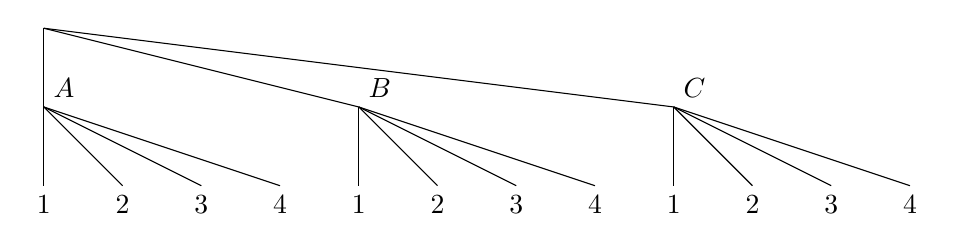
\begin{tikzpicture}
	\draw (0,0)--(0,-1) node[above right] {$A$};
	\draw (0,0)--(4,-1) node[above right] {$B$};
	\draw (0,0)--(8,-1) node[above right] {$C$};
	\draw (0,-1)--(0,-2) node[below] {$1$};
	\draw (0,-1)--(1,-2) node[below] {$2$};
	\draw (0,-1)--(2,-2) node[below] {$3$};
	\draw (0,-1)--(3,-2) node[below] {$4$};
	\draw (4,-1)--(4,-2) node[below] {$1$};
	\draw (4,-1)--(5,-2) node[below] {$2$};
	\draw (4,-1)--(6,-2) node[below] {$3$};
	\draw (4,-1)--(7,-2) node[below] {$4$};
	\draw (8,-1)--(8,-2) node[below] {$1$};
	\draw (8,-1)--(9,-2) node[below] {$2$};
	\draw (8,-1)--(10,-2) node[below] {$3$};
	\draw (8,-1)--(11,-2) node[below] {$4$};
\end{tikzpicture}
We can tell that each branch of the tree gives a different plan, and this list all of them, so we can count the bottom part of the tree to see that there are 12 possibilities. \\

Drawing this tree was a little time consuming and tedious, so we want a general way to do these sort of things. For this type of question we can use the multiplication principle.\\
\textbf{Multiplication Principle:} Suppose that a task is composed of two consecutive choices. If choice 1 can be performed in $m$ ways and for each of those choices, choice 2 can be performed in $n$ different ways, then the complete task can be performed in $m\cdot n$ different ways.\\

In the previous example we can see there are 3 choices for the first flight, and each choice of first flight has 4 choices for the second flight, so there are $3\cdot 4=12$ possible travel plans.\\

Example: Suppose a committee of 10 people needs to choose a president and vice president. How many ways can this be done?\\
We can choose president and vice president in order. First we choose the president and there are 10 choices. Once the president has been chosen, they cannot be chosen for the vice president, so there are 9 possible choices. Thus there are $10\cdot 9=90$ possibilities.\\

Let's make 2 notes about the multiplication principle. First of all, it is very important that each option leads to the same number of possibilites. However, they do not need to be the \underline{same} options. In the previous example the actual choices for vice presient were different, but the number of choices were the same.\\

What if there are more choices?\\
Example: A sub shop allows you to make your own sub by choosing a meat, cheese and a veggie. (Its not a very good sub shop) The choices for meat are ham, turkey, and salami. The cheese choices are swiss, provolone, pepper jack, and american. The veggie choices are letuce, tomato, pickles, peppers and cucumber. How many different subs can you make?\\

Using the multiplication principle, we know that there are $3\cdot 4=12$ possibilites for choosing meat and cheese. What if we think about these two choices as 1 choice with 12 possibilites. Then we have to choose our meat and cheese combo and then our veggie. Then there are $12\cdot 5=60$ possibilites for how to make a sub.\\

This gives us the following rule:
\textbf{Generalized Multiplicaiton Principle:} Suppose a task consists of $t$ choices performed consecutively. Suppose that choice 1 can be performed in $m_1$ ways; for each of these, choice 2 can be performed in $m_2$ ways; choice 3 performed in $m_3$ ways and so forth. Then the task can be performed in $m_1\cdot m_2\cdots m_t$ ways.\\

Example: 6 friends want to take a graduation picture where they stand in a line from left to right. How many possible orders can they stand in?\\
There are 6 choices for the first person in the line. Then there are 5 choices for the next person. Then 4 choices and so forth till there is only one choice for the last person. Thus there are $6\cdot 5\cdot 4\cdot 3\cdot 2\cdot 1=720$ possible orders.\\

The previous situation is so common that it has its own notation. For a positive integer $n$ we define the \defn{factorial} $n!$ to be $n!=n\cdot (n-1)\cdot (n-2)\cdots 2\cdot 1.$ We also adopt the convention that $0!=1.$

Example:\\
A company gives each employee a 3 letter pin. How many possible pins are there? What if they are not allowed to assign pins which are all the same letter? How many such pins are there? Can we use the multiplication principle?

\end{document}
